\documentclass{source/Report}

\major{地理信息科学}
\name{陈杰伟}
\title{RV64 时钟中断}
\stuid{3200101205}
\college{地球科学学院}
\date{\today}
\lab{玉泉曹光彪-西503}
\course{操作系统}
\instructor{寿黎但}
\grades{}
\expname{RV64 时钟中断}
\exptype{编程实验}
\partner{无}

\begin{document}
\makecover
\makeheader
\section{实验目的}
- 学习 RISC-V 的 trap 处理相关寄存器与指令,完成对 trap 处理的初始化。

- 理解 CPU 上下文切换机制,并正确实现上下文切换功能。

- 编写 trap 处理函数,完成对特定 trap 的处理。

- 调用 OpenSBI 提供的接口,完成对时钟中断事件的设置。

\section{实验环境}
Ubuntu 20.04

\section{实验步骤}
\subsection{开启 trap 处理}

设置 stvec, 将 \_traps所表示的地址写入 stvec,采用 Direct模式, 而 traps 则是 trap 处理入口函数的基地址。

\begin{lstlisting}[language = bash, title = {将\_traps的地址写入stvec}]
    # 将_traps的地址写入stvec
    la t0, _traps
    csrw stvec, t0
\end{lstlisting}

将\_traps的地址写入stvec

\begin{lstlisting}[language = bash, title = {启动时钟中断}]
    # 设置 sie[STIE] = 1 是s-mode下时钟中断enable比特位, 启动时钟中断
    csrr t0, sie
    ori t0, t0, 32
    csrw sie, t0
\end{lstlisting}

设置第一次时钟中断,将a2寄存器使用rdtime伪指令存入当前时间作为时钟中断时间,其他参数设为0,调用sbi\_call函数,启动第一次时钟中断

\begin{lstlisting}[language = bash, title = {设置第一次时钟中断}]
    # 调用c函数sbi_ecall,使用opensbi设置第一次时钟中断时间为当前时间
    li a0, 0x00
    li a1, 0x0
    rdtime a2
    li a3, 0x0
    li a4, 0x0
    li a5, 0x0
    li a6, 0x0
    li a7, 0x0
    call sbi_ecall
\end{lstlisting}

开启 S 态下的中断响应, 将 sstatus[SIE]置 1。

\begin{lstlisting}[language = bash, title = {开启 S 态下的中断响应}]
    # 设置 sstatus[SIE] = 1, 在S-mode下开启所有中断
    csrr t0, sstatus
    ori t0, t0, 2
    csrw sstatus, t0
\end{lstlisting}

\subsection{实现上下文切换}

在 arch/riscv/kernel/ 目录下添加 entry.S 文件。

保存 CPU 的寄存器(上下文)到内存中(栈上),使用sd指令保存到程序栈上并更新sp的值,注意最后存入sp到内存

\begin{lstlisting}[language = bash, title = {保存上下文}]
    #该段将32个寄存器和spec的值写入栈中,每个寄存器64位,并随时更新栈顶的地址
    addi sp, sp, -33*16
    sd zero, 0*16(sp)
    sd ra, 1*16(sp)
    sd gp, 2*16(sp)
    sd tp, 3*16(sp)
    sd t0, 4*16(sp)
    sd t1, 5*16(sp)
    sd t2, 6*16(sp)
    sd s0, 7*16(sp)
    sd s1, 8*16(sp)
    sd a0, 9*16(sp)
    sd a1, 31*16(sp)
    sd a2, 10*16(sp)
    sd a3, 11*16(sp)
    sd a4, 12*16(sp)
    sd a5, 13*16(sp)
    sd a6, 14*16(sp)
    sd a7, 15*16(sp)
    sd s2, 16*16(sp)
    sd s3, 17*16(sp)
    sd s4, 18*16(sp)
    sd s5, 19*16(sp)
    sd s6, 20*16(sp)
    sd s7, 21*16(sp)
    sd s8, 22*16(sp)
    sd s9, 23*16(sp)
    sd s10, 24*16(sp)
    sd s11, 25*16(sp)
    sd t3, 26*16(sp)
    sd t4, 27*16(sp)
    sd t5, 28*16(sp)
    sd t6, 29*16(sp)
    csrr t0, sepc+++
    sd t0, 30*16(sp)
    sd sp, 32*16(sp)
\end{lstlisting}

将 scause 和 sepc 中的值传入 trap 处理函数 trap\_handler

\begin{lstlisting}[language = bash, title = {scause 和 sepc 中的值传入 trap 处理函数}]
    # 调用trap_handler启动陷阱事件
    csrr a0, scause
    csrr a1, sepc
    call trap_handle
\end{lstlisting}

在完成对 trap 的处理之后, 从内存中(栈上)恢复CPU的寄存器(上下文)。使用ld指令完成,最先读取sp的值,并恢复sp指向原栈位置。最后使用sret返回spec所指示的中断开始位置

\begin{lstlisting}[language = bash, title = {恢复上下文}]
    #将32个寄存器和spec的值从栈中读取
    ld t0, 30*16(sp)
    csrw sepc, t0
    ld zero, 0*16(sp)
    ld ra, 1*16(sp)
    ld gp, 2*16(sp)
    ld tp, 3*16(sp)
    ld t0, 4*16(sp)
    ld t1, 5*16(sp)
    ld t2, 6*16(sp)
    ld s0, 7*16(sp)
    ld s1, 8*16(sp)
    ld a0, 9*16(sp)
    ld a1, 31*16(sp)
    ld a2, 10*16(sp)
    ld a3, 11*16(sp)
    ld a4, 12*16(sp)
    ld a5, 13*16(sp)
    ld a6, 14*16(sp)
    ld a7, 15*16(sp)
    ld s2, 16*16(sp)
    ld s3, 17*16(sp)
    ld s4, 18*16(sp)
    ld s5, 19*16(sp)
    ld s6, 20*16(sp)
    ld s7, 21*16(sp)
    ld s8, 22*16(sp)
    ld s9, 23*16(sp)
    ld s10, 24*16(sp)
    ld s11, 25*16(sp)
    ld t3, 26*16(sp)
    ld t4, 27*16(sp)
    ld t5, 28*16(sp)
    ld t6, 29*16(sp)
    ld sp, 32*16(sp)
    addi sp, sp, 33*16

    sret #一定要用sret返回sepc地址!!!
\end{lstlisting}

\subsection{实现 trap 处理函数}

在 arch/riscv/kernel/目录下添加 trap.c文件。

实现 trap 处理函数 trap\_handler()

\begin{lstlisting}[language = c, title = {trap\_handler}]
    // scause trap类型 sepc trap发生的地址
    void trap_handler(uint64 scause, uint64 sepc)
    {
        printk("kernel is running!\n"); //指示操作系统陷阱机制运行的输出
    
        uint64 interrupt_sign = scause >> 63;         //获取最高位(interrupt指示位)的值
        uint64 interrupt_type = (scause << 60) >> 60; //获取最低4位(interrupt类型指示位)的值
    
        if (interrupt_sign) // interrupt
        {
            switch (interrupt_type)
            {
            case 5:
                printk("[S] Supervisor Mode Timer Interrupt\n"); //指示发生时钟中断的输出
                clock_set_next_event();
                break;
            default:
                break;
            }
        }
        else // exception
        {
        }
    
        return;
    }
\end{lstlisting}

接受时钟中断传入的scause,sepc寄存器的值

使用位运算获取scause最高位和最低4位的值

最高位1代表发生interrupt,0代表发生exception

最低四位的值为5代表发生时钟中断,打印相关信息并设置下一次时钟中断

\subsection{实现时钟中断相关函数}

在 arch/riscv/kernel/ 目录下添加 clock.c 文件。

在 clock.c 中实现 get\_cycles ( ) : 使用 rdtime汇编指令获得当前 time 寄存器中的值。

\begin{lstlisting}[language = c, title = {get\_cycles}]
    uint64 get_cycles()
    {
        register uint64 time = 0;
        __asm__ volatile(
            "rdtime %[time]\n"
    
            : [time] "=r"(time)
    
            :
    
            : "memory");
    
        return time;
    }
\end{lstlisting}

在 clock.c 中实现 clock\_set\_next\_event ( ) : 调用 sbi\_ecall,设置下一个时钟中断事件。

\begin{lstlisting}[language = c, title = {clock\_set\_next\_event}]
    void clock_set_next_event()
    {
        // 下一次 时钟中断 的时间点
        uint64 next = get_cycles() + TIMECLOCK;
    
        sbi_ecall(0x0, 0x00, next, 0, 0, 0, 0, 0); //调用ecall
    
        return;
    }
\end{lstlisting}

\subsection{运行结果}

运行结果如图1,时钟中断每隔一秒触发一次,功能正确

\begin{figure}[p]
    \centering
    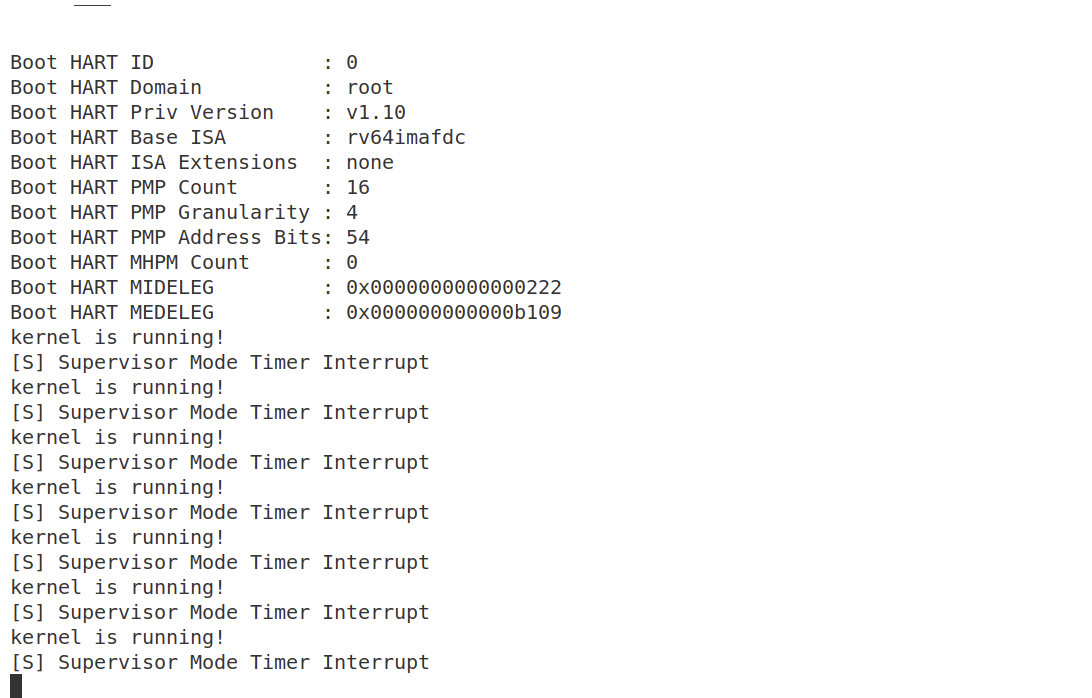
\includegraphics[width = 1\textwidth]{1}
    \caption{运行结果}
\end{figure}


\section{思考题}

1.通过查看 RISC-V Privileged Spec 中的 medeleg 和 mideleg解释上面 MIDELEG 值的含义。

从RISC-V的预设行为来看,所有的interrupt与exception都会在M模式处理,这样显然不够高效,这两个寄存器就代表是否可以委派中断和异常到S模式处理

MIDELEG为222(0010 0010 0010)的含义是

软件、时钟、外部中断全部交到S模式处理

\end{document}

